\documentclass[xcolor=dvipsnames,xcolor=table]{beamer}

\newcommand*{\tcircle}[1]{\tikz[anchor=base,baseline=-2.5pt] \node[circle,fill=#1,scale=0.9] (X) {};}
\newcommand*{\tsquare}[1]{\tikz[anchor=base,baseline=-2.5pt] \node[fill=#1,scale=1.2] (X) {};}
\newcommand*{\tdiamond}[1]{\tikz[anchor=base,baseline=-2.5pt] \node[diamond,fill=#1,scale=0.7] (X) {};}
\newcommand*{\ttriangle}[1]{\tikz[anchor=base,baseline=-1.5pt] \node[regular polygon,regular polygon sides=3,fill=#1,scale=0.6] (X) {};}

\usepackage{tikz}
\usetikzlibrary{shapes.geometric}

\usepackage{tabularx,booktabs}
\newcommand{\camelabr}[2]{{\small #1}{\textsc{#2}}}
\newcommand{\triviaqa}{\camelabr{Trivia}{qa}}
\usepackage[dvipsnames,table]{xcolor}

\usetheme[
          showdate=false,                     % show the date on the title page
          alternativetitlepage=true,         % Use the fancy title page.
          titlepagelogo=general_figures/shell,              % Logo for the fir\
st page.
          ]{UMD}


          \newcommand{\citename}[1]{\small{#1}}

\newcommand{\fsi}[2]{
\begin{frame}[plain]
\vspace*{-1pt}
\makebox[\linewidth]{\includegraphics[width=\paperwidth]{#1}}
\begin{center}
#2
\end{center}
\end{frame}
}

\newenvironment{variableblock}[2]{%
  \setbeamercolor{block body}{#2}
  \begin{block}{#1}}{\end{block}}

\newcommand{\gfxq}[2]{
\begin{center}
	\includegraphics[width=#2\linewidth]{qb/#1}
\end{center}
}

\newcommand{\gfxcm}[2]{
\begin{center}
	\includegraphics[width=#2\linewidth]{qb/cranfield_manchester/#1}
\end{center}
}

\newcommand{\cbcol}[1]{\multicolumn{1}{c}{\textbf{#1}}}

\newcommand{\qb}[0]{\textsc{qb}}
\newcommand{\qa}[0]{\textsc{qa}}
\newcommand{\odqa}[0]{\textsc{odqa}}
\newcommand{\squad}{\textsc{sq}{\small u}\textsc{ad}}
\newcommand{\nq}[0]{\textsc{nq}}
\usepackage{multirow}


\newcommand{\goodbad}[2]{

\begin{columns}

  \column{.5\linewidth}

\begin{variableblock}{Good}{bg=PineGreen,fg=white}
  #1
\end{variableblock}


  \column{.5\linewidth}

\begin{variableblock}{Bad}{bg=BrickRed,fg=white}
  #2
\end{variableblock}


\end{columns}

}


\title[HCQA]{Comparing and Augmenting Human and Computer Intelligence through Natural Language Question Answering}
\author{Jordan Boyd-Graber et al.}
\date{2021}

%gets rid of bottom navigation bars
\setbeamertemplate{footline}[frame number]{}

%gets rid of bottom navigation symbols
\setbeamertemplate{navigation symbols}{}

%gets rid of footer
%will override 'frame number' instruction above
%comment out to revert to previous/default definitions
\setbeamertemplate{footline}{}


\begin{document}

\begin{frame}
  \titlepage{} 
\end{frame}


\begin{frame}{Agenda}

  \begin{itemize}
  \item Problems with Existing QA datasets
  \item Potential Collaboration: Adversarial \textsc{odqa}
  \item Competition: \textsc{qa} and question writing
  \end{itemize}

\end{frame}


\begin{frame}{Google's Natural Questions}
  \only<1>{\gfxq{natural_questions}{1.0}}
  \only<2>{\gfxq{abraham}{1.0}}

  Kwiatkowski et al., 2019
\end{frame}

\fsi{qb/hcqa_ambigqa}{}

\begin{frame}{Ambiguous Questions}
  \rowcolors{2}{gray!25}{white}
  \begin{small}
  \begin{tabular}{p{7cm}p{3cm}}
    \toprule
    Question & Gold Answer \\
    \hline
    \alert<2>{when was the last time michigan won the championship} & 1989 \\
    \alert<3>{what year did the us hockey team won the olympics} & 1960 and 1980 \\
    \alert<4>{which supreme court judge has surved in international court of justice} & Dalveer Bhandari \\
    \alert<5>{where does puerto rico's power come from} & Puerto Rico Electric Power Authority \\
    \bottomrule
  \end{tabular}
  \end{small}
  \begin{block}{Assumptions\dots}
  \only<2>{NCAA Division I Men's Football}
  \only<3>{Men's competition}
  \only<4>{Indian Supreme Court}
  \only<5>{Electric power}
  \only<6>{Bias for Men's sports, especially football.  Ambiguity is arbitrarily resolved by search engine result.}
  \end{block}
\end{frame}



\fsi{qb/hcqa_trivia}{}


\begin{frame}{The problem of ambiguity and annotation error}
  \only<1>{\gfxq{error_and_difficulty_0}{1.0}}
  \only<2>{\gfxq{error_and_difficulty_1}{1.0}}
  \only<3>{\gfxq{error_and_difficulty_2}{1.0}}
  \only<4>{\gfxq{error_and_difficulty_3}{1.0}}

\end{frame}


\begin{frame}{Representation}

      \resizebox{\linewidth}{!}{%
        \begin{tabular}{cl*{8}{r}}
        % \hline
        % \multicolumn{2}{c}{\small{\textbf{Demography}}}  & \textbf{\nq} & \textbf{\qb} & \textbf{\squad} & \textbf{\triviaqa} \\
        \hspace{15pt} & \multirow{2}{*}{\textbf{Value}} %{\small{\textbf{Value}}}  
            & \multicolumn{2}{c}{\textbf{\nq}} 
            & \multicolumn{2}{c}{\textbf{\qb}}  
            & \multicolumn{2}{c}{\textbf{\squad}}  
            & \multicolumn{2}{c}{\textbf{\triviaqa}} \\ 
        & 
            & \cbcol{Train} & \cbcol{Dev}
            & \cbcol{Train} & \cbcol{Dev} 
            & \cbcol{Train} & \cbcol{Dev} 
            & \cbcol{Train} & \cbcol{Dev}\\         
        \toprule
        \multirow{3}{*}{\rotatebox[origin=c]{90}{\textbf{Gender}}}
            & Male    
                &  75.67 &  76.33 
                &  91.77 &  91.63 
                &  87.82 &  95.15 
                &  83.76 &  83.32 \\
               
            & Female          
                &  27.47 &  27.56 
                &  10.29 &   9.87 
                &  13.44 &   5.20 
                &  20.54 &  20.29 \\
                
                % &   0.31 &   0.35 &   0.27 &   0.30
            % & Other           &   0.12 &   0.00 &   0.09 &   0.12 \\
            & No Gender
                &   0.31  &   0.47
        		&   0.35  &   0.39
        		&   0.27  &   0.00
        		&   0.30  &   0.35 \\
        \midrule
        \multirow{6}{*}{\rotatebox[origin=c]{90}{\textbf{Country}}}
            & US
                & 59.62	& 58.66
        		& 29.70	& 26.28
        		& 32.74	& 24.93
        		& 31.32	& 30.91
                \\
            
            & UK
        		& 15.76	& 15.78
        		& 17.92	& 17.68
        		& 19.66	& 16.83
        		& 41.92	& 41.32
        		\\
            
            & France
        		& 1.79	& 1.18
        		& 10.06	& 10.34
        		& 7.76	& 10.57
        		& 4.37	& 4.84
        		\\
            
            & Italy
				& 1.83	& 1.88
				& 8.07	& 10.50
				& 9.00	& 3.88
				& 3.75	& 3.48
				\\
            & Germany        
				& 1.52	& 2.12
				& 7.21	& 6.71
				& 4.77	& 6.61
				& 3.01	& 3.00
				\\

            & No country 
				& 4.82	& 4.36
				& 7.12	& 6.79
				& 3.48	& 2.56
				& 6.19	& 6.10
				\\

        \midrule
        \multirow{7}{*}{\rotatebox[origin=c]{90}{\textbf{Professional Field}}}
            & Film/TV
				& 39.19	& 37.93
				& 3.16	& 1.89
				& 10.72	& 1.32
				& 20.64	& 20.75
				\\
            
            & Writing 
				& 7.40	& 6.95
				& 36.62	& 36.39
				& 10.46	& 6.70
				& 18.41	& 18.05
				\\
				
            & Politics 
				& 11.98	& 10.84
				& 24.02	& 24.86
				& 36.97	& 46.61
				& 21.18	& 20.72
				\\
				
            & Science/Tech
				& 3.61	& 4.71
				& 8.93	& 7.50
				& 13.67	& 29.60
				& 5.43	& 5.54
				\\
				
            & Music  
				& 24.08	& 23.44
				& 9.51	& 10.73
				& 13.56	& 2.64
				& 16.46	& 17.38
				\\
				
            & Sports
				& 13.69	& 16.49
				& 1.31	& 0.32
				& 2.99	& 1.76
				& 11.03	& 11.19
				\\
				
            & Stage
				& 15.67	& 14.84
				& 1.49	& 1.03
				& 1.21	& 1.23
				& 10.89	& 10.28
				\\
			
			& Artist
				& 1.84	& 2.47
				& 9.17	& 9.00
				& 4.58	& 2.38
				& 5.75	& 5.93
				\\
				
        \bottomrule
        \end{tabular}
    }

\end{frame}



\begin{frame}{Trick me if you can\dots}

  \begin{columns}
    \column{.5\linewidth}

    
\includegraphics[width=.5\linewidth]{general_figures/eric}

    \begin{block}{ Trick Me If You Can: Human-in-the-loop Generation of Adversarial Question Answering Examples}
Eric Wallace, Pedro Rodriguez, Shi Feng, Ikuya Yamada, and Jordan Boyd-Graber. Transactions of the Association of Computational Linguistics, 2019. 

    \end{block}
    
    \column{.5\linewidth}
  \begin{itemize}
  \item Trivia writers create questions
  \item {\bf Current systems} explain why they answer (and when)
  \item Trivia writers make questions difficult for both humans and computers
  \end{itemize}
  \end{columns}
\end{frame}

% \begin{frame}{What do we mean by ``adversarial''?}

%   \gfxq{trick/flow_chart_horizontal_label}{1.0}

%   \begin{itemize}
%     \item Both neural and IR systems
%       \pause
%     \item Reason we need to have good explanations of QA
%   \end{itemize}

% \end{frame}

\fsi{qb/trick/brahms_0}{\href{http://write.qanta.org}{http://write.qanta.org}}
\fsi{qb/trick/brahms_1}{}
\fsi{qb/trick/brahms_2}{}
\fsi{qb/trick/brahms_3}{}
\fsi{qb/trick/brahms_4}{}
\fsi{qb/trick/brahms_5}{}


\fsi{qb/trick/round_one}{Just as easy for humans, harder for computers.}



\begin{frame}{Competition}

  \gfxq{trick/pace}{.8}

\begin{itemize}
  \item December 15 2018: Seven top human teams, fourteen computer teams
  \item Top four teams from each ``division'' faced off against each
    other
    \item 2000 challenging sentences
    \pause
  \item All computer teams lost to human teams
    \pause
  \item But two games were really close; strongest system was based on BERT
  \item YouTube videos (including interviews with question writers): \href{https://go.umd.edu/2018hcqa}{https://go.umd.edu/2018hcqa}
\end{itemize}

\end{frame}

\begin{frame}{NeurIPS 2020 Competition}

  \begin{itemize}
  \item Humans can answer in split second / Computers with 500 MiB
  \item Humans can discuss / Computers with 6 GiB
    \item Humans see evidence / Unlimited computers
  \end{itemize}

  \pause
  Humans won convincingly 73--51
\end{frame}

\fsi{qb/hcqa_neurips_2020}{Question}
\fsi{qb/neurips_hcqa_evidence}{Evidence}

\begin{frame}{Hardest questions}

Only four questions reached Phase~3; these questions that stumped both humans and computers:
\begin{itemize}
    \item Kimi no na wa what does it mean
    \item Who said there are old pilots and there are bold pilots
    \item What is the second largest city in ethiopia
    \item Who said i'll make mincemeat out of you
\end{itemize}
  
\end{frame}

\begin{frame}{Benefits of a Competition}

  \begin{itemize}
  \item Bring community together
  \item Opportunity for education: simple to build competitive system
  \item Force people to look at the data
  \item Fair human comparisons (and understand AI weaknesses)
  \item Slowly increase the difficulty
    \item Fun
  \end{itemize}

\end{frame}

\begin{frame}{Concrete Proposal}

  \begin{itemize}
    \item \textsc{odqa} adversarial interface geared for professional
      trivia writers
    \item Leaderboard for computer teams
    \item Leaderboard for question writers (perhaps in conjunction
      with packet submission human trivia tournament)
    \item Final human--computer competition 
  \end{itemize}

\end{frame}

\begin{frame}{What makes for a good question?}

  \begin{itemize}
  \item Feasible (no cap on probability)
  \item Discriminates humans (shallow slope)
  \item Difficult for computers (high intercept)
  \end{itemize}

\end{frame}


\begin{frame}{A Case for Quizbowl}

  \begin{itemize}
    \item Pyramidality ensures proportion of discriminative questions is near 1.0
    \item Editing process minimizes ambiguities and errors
    \item Clever, inventive writers
    \item Fun for participants and viewers
  \end{itemize}
\end{frame}


\begin{frame}
	\frametitle{This isn't new!}
	\begin{columns}

	\column{.5\linewidth}
	\begin{itemize}
		\item Game called ``quiz bowl''
		\item Two teams play each other
		\begin{itemize}
			\item Moderator reads a question
			\item When a team knows the answer, they signal (``buzz'' in)
			\item If right, they get points; otherwise, rest of the question is read to the other team
		\end{itemize}
		\item Hundreds of teams in the US alone
                \only<2>{\item Example \dots}
	\end{itemize}

	\column{.5\linewidth}
	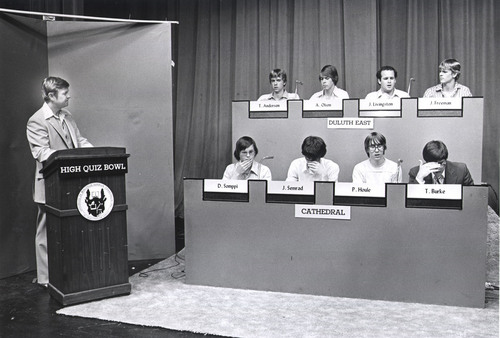
\includegraphics{qb/quizbowl}

	\end{columns}

\end{frame}
\begin{frame}[t]
	\frametitle{Sample Question}

        The Swiss-Italian architect Pietro Antonio Solari
        \only<2->{built several fortified towers in this city, which
          often vied for power with its northern rival Tver. A ruler
          of this city prevailed in the} \only<3->{Great Stand on the
          Ugra River. A prince from this city was nicknamed for
          winning a battle on the} \only<4->{Don river. Partly because
          a ruler of this city married} \only<5->{Sophia Palaiologina,
          the niece of the last Byzantine Emperor, this city styled
          itself the} \only<6->{``Third Rome'' after the fall of
          Constantinople. Another prince of this city stopped paying
          tribute to the} \only<7->{Mongols in 1476, ending the
          ``Tatar yoke.''} \only<8->{The Grand Duchy headquartered in
          this city came to an end in 1547 with the ascension of}
        \only<9->{ Ivan IV, who made it his capital. For 10 points,
          name this city where Ivan III renovated the
          Kremlin,} \only<10->{the capital of Russia.}\\
        \vspace{.5cm} \only<11->{ {\bf Moscow} (Moskva / Muscovy)}

\end{frame}




\begin{frame}{Impossible Until the End}
\alert<3>{Ritchie Watson commended this play's historical accuracy for
  getting the price for a dozen eggs right---ten cents---to defend
  against Elizabeth Hardwick’s contention that it was a sentimental
  history.} \alert<4>{At the end of this play, a man wonders why a wheelchair is
at the top of a staircase, and} \alert<5>{Alexandra announces that she is leaving
her mother. Leo is pressured into stealing a set of valuable railroad
bonds in this drama. In this play, which takes its title from the Song
of Solomon,} Regina Hubbard schemes  \tdiamond{PineGreen}
\tcircle{PineGreen} to obtain a majority share in a cotton mill. For 10
points,  \tsquare{PineGreen}  \ttriangle{PineGreen} name this play by
Lillian Hellman. \\

\pause

\textbf{Answer}: The\ Little\ Foxes\\

\only<3>{Academic literature}
\only<4>{Vague plot summary}
\only<5>{Avoid last names}

\end{frame}

% Tricky and hard: F3 Question 25

\begin{frame}{Tricky and impossible for current systems}
In Our Town, a character  \ttriangle{BrickRed} with this given name explains Grover’s Corners’ place in the universe. In The Crucible, a character  \tcircle{BrickRed} with this first name contends that the girls’ actions are part of their “silly seasons” and is the wife of Francis Nurse. A novel with this name, which conducts hidden messages to Rommel in The English Patient, is titled for a character who is killed in a boating accident at Manderley. For 10 points, give this name of a Daphne du Maurier  \tdiamond{Goldenrod}  \tsquare{PineGreen} gothic novel which is also the first name of Miss Sharp, the protagonist of William Thackeray's Vanity Fair. \tcircle{gray}  \ttriangle{gray}


\ttriangle{BrickRed} Thornton Wilder
\tcircle{BrickRed} Richard
\tcircle{gray} Richard
\ttriangle{gray} Thornton Wilder \\
\textbf{Answer}: Rebecca\\
\end{frame}


\begin{frame}{Close, but \dots}
An army that took its name from this geographical feature had a
British doctor, James Paroissien, as its Surgeon General, and recent
scholarship by Peter Blanchard revealed its use of slaves. That army
crossed this geographical feature according  \ttriangle{BrickRed} to
Thomas Maitland’s  \tcircle{BrickRed} plans at Uspallata and Los
Patos. Spanish forces under Rafael Maroto were defeated in the
foothills of these mountains by an army led by José de San Martín and
Bernardo O'Higgins.  \tsquare{BrickRed} For 10 points, name this mountain
range of South America that played a role  \ttriangle{Goldenrod} in the
independence of Chile. \tdiamond{gray}  \tcircle{gray}  \tsquare{gray}

\ttriangle{BrickRed} Angel Falls
\tcircle{BrickRed} Mountain
\tsquare{BrickRed} Battle of Chacabuco
\tdiamond{gray} Battle of Chacabuco
\tcircle{gray} Mountain
\tsquare{gray} Battle of Chacabuco \\
\pause
\textbf{Answer}: Andes\\

\end{frame}


\begin{frame}{Linguistics FTW}

  The main character of a story by \alert<2>{this author opens Crime and Punishment} to a
random page, but finds it to be a copy of The Brother Karamazov, and equates
himself with Monsieur Bovary. This author wrote a story in which the priest
Naigu undergoes a boiling treatment to decrease the size of his nose. This
author of "Cogwheels" wrote about two people who steal to survive near the
southern gate of Kyoto in a story that features inconsistent accounts from a
woodcutter, a priest, a widow, and the ghost of a samurai. For 10 points, name
this author of "Rashomon" and namesake of a Japanese literary prize. \\
\only<3->{\textbf{Answer}: Ryunosuke Akutagawa}
\end{frame}




\begin{frame}{Sabotaged by IR}

  \rowcolors{2}{gray!25}{white}
  \begin{small}
  \begin{tabular}{p{7cm}p{3cm}}
    \toprule
    Question & Page \\
    \hline
 when did the states secede during the civil war &  Border states (American Civil War) \\
 who wears number 2 for the dallas cowboys &  Jeff Heath (American football) \\
 how many countries participated for the first time in the 2014 olympic winter games in sochi & 2014 Winter Paralympics \\
 game of thrones season 7 number of episoded &  List of Teen Wolf episodes \\
 \bottomrule
  \end{tabular}
  \end{small}

\end{frame}

\begin{frame}{Good for Search, Bad for QA}

  Title of page is answer, annotators didn't find span:
  \rowcolors{2}{gray!25}{white}
  \begin{tabular}{p{7cm}p{3cm}}
    \toprule
    Question & Page \\
    \hline
  who plays the goblin king in the hobbit &  Barry Humphries  \\
  who does the voice of fart in rick and morty & Jemaine Clement   \\
 \bottomrule
  \end{tabular}
\end{frame}

\begin{frame}{Questions Depends on Who / When}
  \rowcolors{2}{gray!25}{white}
  \begin{tabular}{p{8cm}p{2cm}}
    \toprule
    Question & Gold Answer \\
    \hline
    can i buy wine in kentucky on sunday & --- \\
    where am i on the steelers waiting list & --- \\
    when is the real housewives on & --- \\
    who has majority in the house and senate & --- \\
    \bottomrule
  \end{tabular}  

  \pause

  \begin{block}{Answerable Questions\dots}
  But depend on which county of Kentucky you're in,
  when you paid for your season pass, and the local network
  syndicating Real Housewives.
  \end{block}
  
\end{frame}



\fsi{qb/jeopardy}{IBM Watson: QA Solved!}

\fsi{qb/kennings-goat}{2020}

\begin{frame}{But is Jeopardy! about Knowledge?}

  \begin{columns}
    \column{.25\linewidth}
    \gfxq{planet_money}{.75}
    \gfxq{jennings}{.7}  
    \gfxq{kenny_malone}{.7}
    \column{.7\linewidth}

    From \href{file:///Users/jbg/repositories/jbg-talks/qb/jennings-buzzer.mp3}{Planet Money} \\
    
    \small

    {\bf JENNINGS:} The deal with the buzzer is this. The buzzer is
    not live until Alex finishes reading the question. And if you buzz
    in before your buzzer goes live, \alert<1>{you actually lock yourself out
    for a fraction of a second}. So the big mistake on the show is
    people who are all adrenalized and are buzzing too quickly, too
    eagerly.

    \pause

    {\bf MALONE:} OK. To some degree, "Jeopardy!" is kind of a video game, and a \alert<2>{crappy video game where it's, like, light goes on, press button} - that's it.

    \pause
    
    {\bf JENNINGS:} (Laughter) Yeah.

    {\bf MALONE:} Is that true?

    {\bf JENNINGS:} I do like to think of it as a \alert<3>{beautiful art} and not a really crappy video game.
    
  \end{columns}
  
\end{frame}


\begin{frame}{References}
\bibliographystyle{style/acl}
\tiny
\bibliography{bib/journal-full,bib/jbg}
\end{frame}



\end{document}
